% Options for packages loaded elsewhere
\PassOptionsToPackage{unicode}{hyperref}
\PassOptionsToPackage{hyphens}{url}
\PassOptionsToPackage{dvipsnames,svgnames,x11names}{xcolor}
%
\documentclass[
  letterpaper,
  DIV=11,
  numbers=noendperiod]{scrartcl}

\usepackage{amsmath,amssymb}
\usepackage{iftex}
\ifPDFTeX
  \usepackage[T1]{fontenc}
  \usepackage[utf8]{inputenc}
  \usepackage{textcomp} % provide euro and other symbols
\else % if luatex or xetex
  \usepackage{unicode-math}
  \defaultfontfeatures{Scale=MatchLowercase}
  \defaultfontfeatures[\rmfamily]{Ligatures=TeX,Scale=1}
\fi
\usepackage{lmodern}
\ifPDFTeX\else  
    % xetex/luatex font selection
\fi
% Use upquote if available, for straight quotes in verbatim environments
\IfFileExists{upquote.sty}{\usepackage{upquote}}{}
\IfFileExists{microtype.sty}{% use microtype if available
  \usepackage[]{microtype}
  \UseMicrotypeSet[protrusion]{basicmath} % disable protrusion for tt fonts
}{}
\makeatletter
\@ifundefined{KOMAClassName}{% if non-KOMA class
  \IfFileExists{parskip.sty}{%
    \usepackage{parskip}
  }{% else
    \setlength{\parindent}{0pt}
    \setlength{\parskip}{6pt plus 2pt minus 1pt}}
}{% if KOMA class
  \KOMAoptions{parskip=half}}
\makeatother
\usepackage{xcolor}
\setlength{\emergencystretch}{3em} % prevent overfull lines
\setcounter{secnumdepth}{5}
% Make \paragraph and \subparagraph free-standing
\ifx\paragraph\undefined\else
  \let\oldparagraph\paragraph
  \renewcommand{\paragraph}[1]{\oldparagraph{#1}\mbox{}}
\fi
\ifx\subparagraph\undefined\else
  \let\oldsubparagraph\subparagraph
  \renewcommand{\subparagraph}[1]{\oldsubparagraph{#1}\mbox{}}
\fi


\providecommand{\tightlist}{%
  \setlength{\itemsep}{0pt}\setlength{\parskip}{0pt}}\usepackage{longtable,booktabs,array}
\usepackage{calc} % for calculating minipage widths
% Correct order of tables after \paragraph or \subparagraph
\usepackage{etoolbox}
\makeatletter
\patchcmd\longtable{\par}{\if@noskipsec\mbox{}\fi\par}{}{}
\makeatother
% Allow footnotes in longtable head/foot
\IfFileExists{footnotehyper.sty}{\usepackage{footnotehyper}}{\usepackage{footnote}}
\makesavenoteenv{longtable}
\usepackage{graphicx}
\makeatletter
\def\maxwidth{\ifdim\Gin@nat@width>\linewidth\linewidth\else\Gin@nat@width\fi}
\def\maxheight{\ifdim\Gin@nat@height>\textheight\textheight\else\Gin@nat@height\fi}
\makeatother
% Scale images if necessary, so that they will not overflow the page
% margins by default, and it is still possible to overwrite the defaults
% using explicit options in \includegraphics[width, height, ...]{}
\setkeys{Gin}{width=\maxwidth,height=\maxheight,keepaspectratio}
% Set default figure placement to htbp
\makeatletter
\def\fps@figure{htbp}
\makeatother

\KOMAoption{captions}{tableheading}
\makeatletter
\@ifpackageloaded{caption}{}{\usepackage{caption}}
\AtBeginDocument{%
\ifdefined\contentsname
  \renewcommand*\contentsname{Table of contents}
\else
  \newcommand\contentsname{Table of contents}
\fi
\ifdefined\listfigurename
  \renewcommand*\listfigurename{List of Figures}
\else
  \newcommand\listfigurename{List of Figures}
\fi
\ifdefined\listtablename
  \renewcommand*\listtablename{List of Tables}
\else
  \newcommand\listtablename{List of Tables}
\fi
\ifdefined\figurename
  \renewcommand*\figurename{Figure}
\else
  \newcommand\figurename{Figure}
\fi
\ifdefined\tablename
  \renewcommand*\tablename{Table}
\else
  \newcommand\tablename{Table}
\fi
}
\@ifpackageloaded{float}{}{\usepackage{float}}
\floatstyle{ruled}
\@ifundefined{c@chapter}{\newfloat{codelisting}{h}{lop}}{\newfloat{codelisting}{h}{lop}[chapter]}
\floatname{codelisting}{Listing}
\newcommand*\listoflistings{\listof{codelisting}{List of Listings}}
\makeatother
\makeatletter
\makeatother
\makeatletter
\@ifpackageloaded{caption}{}{\usepackage{caption}}
\@ifpackageloaded{subcaption}{}{\usepackage{subcaption}}
\makeatother
\ifLuaTeX
  \usepackage{selnolig}  % disable illegal ligatures
\fi
\usepackage{bookmark}

\IfFileExists{xurl.sty}{\usepackage{xurl}}{} % add URL line breaks if available
\urlstyle{same} % disable monospaced font for URLs
\hypersetup{
  pdftitle={Income Disparity and Its Influence on Higher Education Affordability and Access},
  pdfauthor={Michael Fang; Harrison Huang},
  colorlinks=true,
  linkcolor={blue},
  filecolor={Maroon},
  citecolor={Blue},
  urlcolor={Blue},
  pdfcreator={LaTeX via pandoc}}

\title{Income Disparity and Its Influence on Higher Education
Affordability and Access\thanks{Code and data are available at:
https://github.com/fanger2791/College-Tuition-and-Income-Inequality/tree/main}}
\author{Michael Fang \and Harrison Huang}
\date{February 19, 2024}

\begin{document}
\maketitle
\begin{abstract}
Throughout the years, we have seen how rising income inequality fuels
college tuition hikes, casting a spotlight on the urgent need for
policies that bridge the educational divide. This paper is a
reproduction on the connection between rising income inequality and the
surge in college tuition costs in the United States. Utilizing a
detailed economic model, the increasing disparity in income has been a
significant driver behind the growth in tuition fees since 1990,
accounting for more than half of the observed increase and has also led
to a decline in college attendance rates. Extending this analysis
through secondary research to include Canadian universities reveals
similar trends, indicating a broader North American pattern where income
inequality impacts educational accessibility. This comparative approach
underscores the global relevance of their findings, suggesting that
addressing income disparities could play a crucial role in making higher
education more accessible.
\end{abstract}

https://www.aeaweb.org/articles?id=10.1257/aer.20181027

\section{Introduction}\label{introduction}

In recent years, the escalating cost of college tuition in the United
States has emerged as a critical issue, intertwining with the broader
narrative of rising income inequality. The paper by Zhifeng Cai and
Jonathan Heathcote addresses this pressing concern by examining the
relationship between these two phenomena. Utilizing a competitive model
of the college market, the study not only uncovers the mechanisms that
link rising income inequality to increasing tuition costs but also sheds
light on the consequent impacts on college attendance and social
mobility. Through this paper, we aim to illuminate the unique challenges
and opportunities facing the Canadian higher education system in the
context of rising tuition costs and income inequality. Incorporating a
Canadian perspective into our reproduction study adds a crucial
comparative dimension, allowing us to explore the dynamics of university
tuition and income inequality within a different national context. This
extension acknowledges the distinct structure of the Canadian higher
education system and its funding mechanisms, which differ from those in
the United States in terms of government support, the magnitude of
tuition fees, and the socio-economic landscape.

Central to the Zhifeng Cai and Jonathan Heathcote paper's findings is
the assertion that the surge in U.S. income inequality since the 1990s
can account for more than half of the observed increase in average net
tuition over the same period. This relationship underscores a critical
feedback loop where income disparities not only affect individual
capacity to afford higher education but also drive institutional
behaviors around tuition setting. Moreover, the paper highlights the
detrimental effects of rising tuition on college attendance rates,
particularly among lower-income segments, positing significant
implications for social mobility and equity.

To build upon the original work of Zhifeng Cai and Jonathan Heathcote,
our project will undertake a reproduction of the study, focusing on two
or three of its core aspects. This will involve:

\begin{enumerate}
\def\labelenumi{\arabic{enumi}.}
\item
  Recreating Table 3: We will split the table into private college
  versus public college. In the original work, it was not clearly stated
  where the data came from or for private two year studies or public
  four year studies. With that, we will look at data sets from the paper
  and recreate Table 3 from the original work. The new tables will focus
  on the price change from the earliest data and most recent data. In
  addition, the two tables are separated by private four year non profit
  college versus public four year college. This step includes extensive
  data cleaning and edits due to excel file formats. All the steps can
  be found in the source code to increase the reproducibility of our
  analysis.
\item
  Recreating the Model: We will start by reproducing the competitive
  college market model used in the original study, ensuring our work is
  entirely reproducible. This step includes verifying the model's
  assumptions, computational methods, and data inputs.
\item
  Expanding the Study with a Canadian Lens: Specifically examine how
  income inequality within Canada affects university tuition, comparing
  these dynamics with the findings from the U.S. context. This will
  provide insights into how different policy environments and
  socio-economic conditions influence the relationship between income
  inequality and higher education costs.
\end{enumerate}

Our project involves crafting a concise paper that encapsulates the
entire reproduction study. This paper will meticulously outline our
source and methodology, ensuring clarity on how we've mirrored the
original study's model while integrating steps for high reproducibility.
It will also present a comparative analysis of our findings against the
original study's conclusions, pinpointing any variances and their
potential causes. Additionally, the paper will delve into the
implications of our policy simulations, offering insights into how
income inequality influences college tuition and attendance. Lastly, it
will propose directions for future research, highlighting areas within
the college tuition-income inequality nexus that remain unexplored,
setting the stage for subsequent scholarly inquiry.

\section{Data}\label{sec-data}

\subsection{Source}\label{source}

\subsection{Methodology}\label{methodology}

In replicating the original model by Zhifeng Cai and Jonathan Heathcote,
our methodology was meticulously crafted to mirror their approach with
precision, ensuring the highest degree of reproducibility. This entailed
a thorough analysis of the original study's model, including its
assumptions, variables, and computational methods. We closely followed
the procedural steps outlined in their research, from data collection
through to the analytical techniques employed to examine the
relationship between income inequality and college tuition costs. To
guarantee reproducibility, we documented each step of our process in
detail, including the coding practices, statistical software used, and
the sources of our data. This approach not only underscores our
commitment to transparency and scientific integrity but also enhances
the reliability of our replication efforts.

R was the language and environment used for the bulk of this
reproduction, alongside

\subsection{Features}\label{features}

\section{Results}\label{results}

\subsection{Public Four Year College
Data}\label{public-four-year-college-data}

\begin{longtable}[]{@{}
  >{\raggedright\arraybackslash}p{(\columnwidth - 8\tabcolsep) * \real{0.5444}}
  >{\raggedright\arraybackslash}p{(\columnwidth - 8\tabcolsep) * \real{0.0778}}
  >{\raggedright\arraybackslash}p{(\columnwidth - 8\tabcolsep) * \real{0.0778}}
  >{\raggedright\arraybackslash}p{(\columnwidth - 8\tabcolsep) * \real{0.1556}}
  >{\raggedright\arraybackslash}p{(\columnwidth - 8\tabcolsep) * \real{0.1444}}@{}}

\caption{\label{tbl-public\_data}Public Four Year College Data}

\tabularnewline

\toprule\noalign{}
\begin{minipage}[b]{\linewidth}\raggedright
Type
\end{minipage} & \begin{minipage}[b]{\linewidth}\raggedright
Data\_1
\end{minipage} & \begin{minipage}[b]{\linewidth}\raggedright
Data\_2
\end{minipage} & \begin{minipage}[b]{\linewidth}\raggedright
PercentChange
\end{minipage} & \begin{minipage}[b]{\linewidth}\raggedright
TimeFrame
\end{minipage} \\
\midrule\noalign{}
\endhead
\bottomrule\noalign{}
\endlastfoot
Net TFRB & 8730 & 14210 & 62.77\% & 1996 to 2016 \\
Grants by Income(1) & 5847 & 9835 & 68.21\% & 1999 to 2011 \\
Grants by Income(2) & 3693 & 6667 & 80.53\% & 1999 to 2011 \\
Grants by Income(3) & 1748 & 2967 & 69.74\% & 1999 to 2011 \\
Grants by Income(4) & 1443 & 2576 & 78.52\% & 1999 to 2011 \\
Funding for Higher Education per 1000\$ of Income & 7.37 & 5.283 &
-28.31\% & 1984 to 2014 \\
Tuition Revanue & 6610 & 9740 & 47.35\% & 2003 to 2013 \\
Subsidy & 8350 & 7640 & -8.5\% & 2003 to 2013 \\

\end{longtable}

\subsection{Private Four Year College
Data}\label{private-four-year-college-data}

\begin{longtable}[]{@{}
  >{\raggedright\arraybackslash}p{(\columnwidth - 8\tabcolsep) * \real{0.5444}}
  >{\raggedright\arraybackslash}p{(\columnwidth - 8\tabcolsep) * \real{0.0778}}
  >{\raggedright\arraybackslash}p{(\columnwidth - 8\tabcolsep) * \real{0.0778}}
  >{\raggedright\arraybackslash}p{(\columnwidth - 8\tabcolsep) * \real{0.1556}}
  >{\raggedright\arraybackslash}p{(\columnwidth - 8\tabcolsep) * \real{0.1444}}@{}}

\caption{\label{tbl-private\_data}Private Four Year College Data}

\tabularnewline

\toprule\noalign{}
\begin{minipage}[b]{\linewidth}\raggedright
Type
\end{minipage} & \begin{minipage}[b]{\linewidth}\raggedright
Data\_1
\end{minipage} & \begin{minipage}[b]{\linewidth}\raggedright
Data\_2
\end{minipage} & \begin{minipage}[b]{\linewidth}\raggedright
PercentChange
\end{minipage} & \begin{minipage}[b]{\linewidth}\raggedright
YearFrame
\end{minipage} \\
\midrule\noalign{}
\endhead
\bottomrule\noalign{}
\endlastfoot
Net TFRB & 20020 & 26080 & 30.27\% & 1996 to 2016 \\
Grants by Income(1) & 12155 & 22827 & 120\% & 1999 to 2011 \\
Grants by Income(2) & 11821 & 20355 & 80.84\% & 1999 to 2011 \\
Grants by Income(3) & 10333 & 15389 & 28.30\% & 1999 to 2011 \\
Grants by Income(4) & 6328 & 12489 & 97.36\% & 1999 to 2011 \\
Funding for Higher Education per 1000\$ of Income & 7.37 & 5.283 &
-28.31\% & 1984 to 2014 \\
Tuition Revanue & 19860 & 23360 & 17.62\% & 2003 to 2013 \\
Subsidy & 15560 & 20050 & 28.86\% & 2003 to 2013 \\

\end{longtable}

In the two tables Table~\ref{tbl-public_data} and
Table~\ref{tbl-private_data}, the first column stands for tuition, fees,
room and board. This is a summary data of the entire expense at that
specific institution. The Grants by Income data then looks grants by
year given to each income group. For example, the second row of the
table looks at grants given out to people that has an annual income of
less than 30,000. The sixth row looks at state funding according to an
individual's income by per 1000. For example, if an individual were to
make 50,000 a year, state funding for higher education to that
individual should be 368.5\$. There was no private and public data, as a
result the state funding data is the same for both private and public
colleges. The last two row looks at the data of the institution's
revenue and expenditure on subsidizing students. The year frame was
different for each data sets, therefore, we decided to create a separate
column for cleaner look for the table. This would prevent N/A cells and
could be confusing for readers.

First, looking at Table~\ref{tbl-public_data}, there is a big increase
in the net fees at 62.77\% increase in just 20 years. Then looking at
the grants given out by the public institutions, even though we see a
continuous increase of more funding for the two lower income groups, we
are still seeing a big increase in percentage for higher income
individuals. When looking at state funding, there is even a -28.31 \%
decrease in the funding for higher education. Lastly looking at the
tuition revenue and subsidy, despite making steady profits, the
institution on the other hand decreased subsitizing expenditures by
8.5\% from 2003 to 2014.

Second, here are some key findings from Table~\ref{tbl-private_data}.
There is a less increase of fees at 30.27\%. However, the total
expenditure is significant more compared to public institutions. Then
looking at the grants given out by private institutions, with the lowest
income group gaining a significant increase of 120\%. Interestingly, the
highest group also gained 97.36\%. In the same situation, state funding,
showed a -28.31 \% decrease for higher education. Lastly looking at the
tuition revenue and subsidy, 17.62\% increase in tuition revenue, and
also an increase of 28.86\% subsidy expenditures.

Comparing the two data set, we can see that even though the percentage
increase of private institution fees. The net expenditure is still
almost three times of public institutions. Overall by income group,
private institutions are also a lot more generous in giving out grants,
with large numbers compared to public institutions. Private institutions
also have a positive percentage increase of subsidy expenditure compared
to public institutions despite both having positive tuition revenue over
the years. From the table, we can see that private institutions are much
more generous in terms of grants and expenditure studies, however, they
are also a lot more expensive to attend compared to public schools.

In attempts to uncover more about income disparity and the accesses of
higher education, we will recreate two models from the paper.

\subsection{College Tuition And Fees}\label{college-tuition-and-fees}

\begin{figure}

\centering{

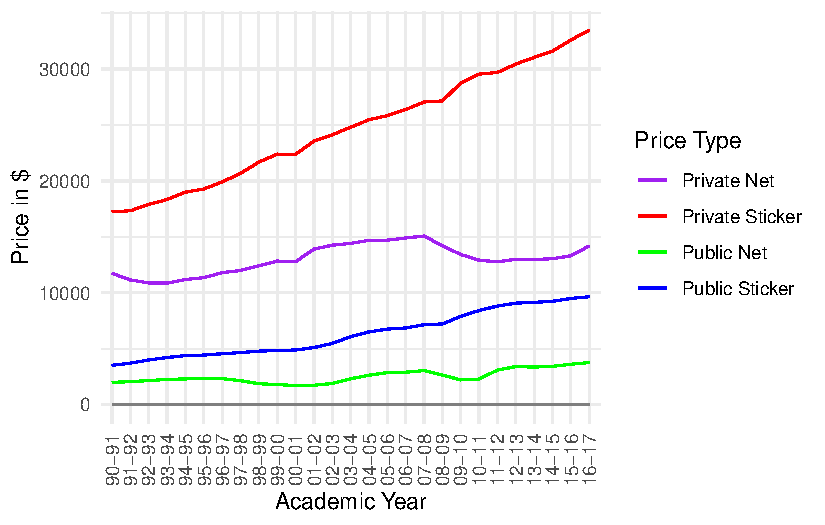
\includegraphics{paper_files/figure-pdf/fig-stickers-1.pdf}

}

\caption{\label{fig-stickers}College Tuition And Fees, US\$(2016)}

\end{figure}%

Figure~\ref{fig-stickers}, as presented, showcases a multi-decade
overview of college tuition and fees in the United States, providing a
clear visual representation of trends across both public and private
institutions, accounting for inflation to 2016 dollars. The graph is
particularly telling in its illustration of the divergent paths between
sticker prices and net prices over time.

The private sticker prices, marked by the red line, demonstrate an
unbroken ascent throughout the years, effectively doubling from the
early 1990s to 2017. This relentless increase is indicative of a higher
education market that is possibly responding to increased demand, or
perhaps reflecting rising costs associated with providing education,
such as faculty salaries, facilities, and resources.

In contrast, the private net prices, shown with the purple line, while
following an upward trajectory, do so with a less pronounced slope. This
implies that financial aid has absorbed some of the shock of rising
sticker prices for students, although it's worth noting that the gap
between sticker and net prices appears to widen over time, suggesting
that financial aid may not be keeping pace with the increases in sticker
prices.

For public institutions, the sticker prices, represented by blue line,
show a significant increase but remain substantially lower than those of
private institutions. This could reflect the impact of state funding and
the different market pressures affecting public colleges and
universities. The relatively gentle slope of the public net prices,
depicted by the green line, indicates a measure of stability in what
students actually pay, possibly due to a combination of state subsidies,
federal aid, and institutional grants.

The stability of public net prices, despite the increase in public
sticker prices, could be seen as a reflection of a commitment to
maintaining access to higher education. However, the upward trend in
both sticker and net prices, even if modest for public institutions,
points to a broader trend of increasing financial burden on students and
families, which may have significant implications for access to higher
education, especially for those from lower-income backgrounds.

Analyzing Figure 1 also prompts consideration of the broader economic
context, including changes in the funding models for higher education,
the role of government policy, and the economic factors at play during
this period, such as recessions and economic booms, which can influence
both the supply and demand sides of higher education. The continuous
rise in prices, especially in the private sector, may also reflect a
competitive market where institutions vie for prestige, faculty, and
facilities, which in turn, raises the question of the true value of
higher education and the return on investment for students.

\subsection{Comparison of Income Distribution for 1989 and
2016}\label{comparison-of-income-distribution-for-1989-and-2016}

\begin{figure}

\centering{

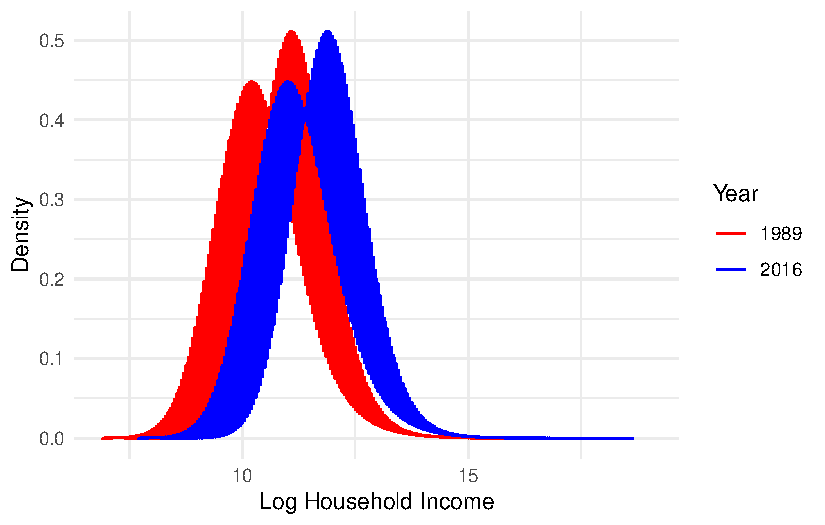
\includegraphics{paper_files/figure-pdf/fig-log-1.pdf}

}

\caption{\label{fig-log}Comparison of Income Distribution for 1989 and
2016}

\end{figure}%

Figure~\ref{fig-log} is a comparison of estimated income distributions
for two different years, 1989 and 2016, represented using a probability
density function on a logarithmic scale for household income.

The x-axis represents the logarithm of household income, indicating that
the data is not raw income but transformed using a logarithmic function,
likely to normalize the distribution and to handle the wide range of
incomes more effectively. The use of logarithms in income distribution
is common as it tends to make the distribution more symmetric and
resemble a normal distribution, which is easier to work with
statistically.

The y-axis represents the density, which is the probability per unit on
the x-axis. In a probability density function, the area under the curve
for a given interval represents the probability that a randomly selected
household will have an income within that interval.

The increase in the variance of log income suggests that income
inequality has widened from 1989 to 2016. This finding correlates with
the hypothesis that growing income inequality might be one of the
drivers behind the increase in college tuition. This could indicate that
while the relative differences in income may have not shifted
dramatically on a logarithmic scale, the actual incomes have grown,
particularly at the higher end, contributing to the right skewness seen
in the 2016 distribution.

\section{Discussion}\label{discussion}

\subsection{Findings}\label{findings}

The paper by Zhifeng Cai and Jonathan Heathcote delves into the nuanced
dynamics between escalating college tuition fees and the widening gap of
income inequality in the United States. It posits a model showcasing how
increased income disparities significantly drive up tuition costs,
thereby impacting college accessibility. The study highlights the
strategic role of financial aid and subsidies in counteracting tuition
hikes, yet underscores their insufficiency in bridging the educational
divide. Through a detailed examination of higher education market
dynamics, the paper sheds light on the competitive practices of
colleges, such as differential pricing and the allocation of financial
aid, aimed at attracting students. This analysis culminates in a
discussion on the broader implications for policy, suggesting that
reform in financial aid structures and a reevaluation of higher
education funding models are imperative to address these challenges. The
findings present a critical perspective on the economic forces shaping
the higher education landscape, offering insights that could guide
policy reforms aimed at ensuring equitable access to college education
amidst growing income inequality.

\subsection{Dynamics of Canadian Universities using insights by Cai and
Heathcote}\label{dynamics-of-canadian-universities-using-insights-by-cai-and-heathcote}

To explore the dynamics of Canadian universities through the insights
provided in the paper by Zhifeng Cai and Jonathan Heathcote and applying
a Canadian lens, it's vital to delve into the nuances of tuition trends,
income inequality, and access to higher education within Canada.
Canadian universities have been experiencing a rise in tuition fees
across various programs, with notable increases in professional degrees
such as dentistry, medicine, law, and engineering, reflecting a
potential barrier to access for students from lower-income backgrounds.
The disparities in tuition fees are further exacerbated when considering
the level of study, with graduate programs generally demanding higher
fees than undergraduate ones, aligning with the expected returns in
terms of future employment income.

The socioeconomic landscape in Canada, marked by growing income
inequality, has profound implications for higher education access and
outcomes. Trends in intergenerational income mobility and income
inequality suggest that the economic background of a student's family
plays a significant role in their educational opportunities and future
earnings, thereby influencing their ability to afford higher education.

Moreover, the stratification of higher education institutions, observed
both in the U.S. and Canada, indicates that access to elite institutions
is highly influenced by social and economic factors. This stratification
is perpetuated by the increasing concentration of resources and student
selectivity at more prestigious universities, further challenging the
meritocratic ideals of higher education.

Canadian higher education is also characterized by regional disparities
in tuition fees and additional compulsory fees, with provinces like
Alberta having higher fees compared to the national average. This
regional variation adds another layer of complexity to the affordability
and accessibility of higher education across the country. The increasing
reliance on international students, who pay significantly higher tuition
fees, further highlights the financial challenges faced by Canadian
universities and the potential impact on domestic students' access to
education.

Addressing these challenges requires a multifaceted approach that
considers the role of public funding, financial aid, and policies aimed
at reducing income inequality and improving access to higher education
for all Canadians. Ensuring that higher education remains a pathway for
social mobility and economic opportunity is crucial in the face of
rising tuition costs and socioeconomic disparities.

\subsection{Potential Weaknessess}\label{potential-weaknessess}

There are several potential weaknesses in the findings that warrant
consideration. Firstly, the model's assumptions, including a continuous
distribution of college quality and linear relationships between
variables, might oversimplify the complex, non-linear dynamics present
in real-world scenarios. This simplification could introduce
inaccuracies in predicting tuition trends and attendance patterns.
Secondly, the study's reliance on observed data trends and specific
calibrations may not fully encapsulate the intricacies of income
distribution, tuition policies, and other socioeconomic factors, leading
to potential biases or limitations in the dataset used for analysis.

Moreover, while the model accounts for a broad spectrum of college
quality, it might not accurately represent specific types of educational
institutions, such as community colleges, vocational schools, and online
universities, which do not adhere to the traditional metrics of college
quality. Additionally, the focus on income inequality as the primary
driver overlooks other significant factors, such as changes in
government funding for education, demographic shifts, and evolving labor
market demands, which could also influence tuition costs and attendance
rates.

Furthermore, the model may not sufficiently consider how policy changes
or shifts in household behavior in response to rising tuition and income
inequality could alter the college market dynamics. For instance, the
increasing prevalence of online education and alternative credentialing
pathways might disrupt traditional patterns of college attendance and
tuition pricing strategies. Lastly, the study's conclusions are based on
historical data up to a certain point, and the long-term applicability
of these findings might be limited by emerging trends and changes in the
landscape of higher education and economic inequality.

\subsection{Limitations to
reproducing}\label{limitations-to-reproducing}

From a reproducibility standpoint, the absence of provided code or
detailed methodology for recreating the tables, graphs, and statistical
analyses by Zhifeng Cai and Jonathan Heathcote introduces significant
limitations. The ability to replicate study findings is foundational to
the validation and advancement of scientific research. Without access to
the exact computational procedures, data analysis scripts, or software
used, other researchers are hindered in their ability to verify the
results, explore the implications further, or apply the methodology to
new datasets. This lack of transparency can impede the reproducing
process as others may struggle to build directly on these findings
without a clear understanding of the original analysis techniques.

Moreover, the reproducibility issue extends beyond just the recreation
of visualizations to the very core of the study's conclusions. The
modeling assumptions, data transformations, and statistical methods
employed are crucial for understanding the dynamics between income
inequality and college tuition. Without clear documentation or code, it
becomes challenging to assess the robustness of the model, the
sensitivity of the results to different assumptions, or the potential
for bias in the analysis. This gap not only affects the credibility of
the findings but also limits the potential for educational policymakers,
economists, and other stakeholders to apply these insights effectively.

\subsection{Future Research}\label{future-research}

Future directions should focus on closing gaps in our understanding of
the dynamics between income inequality and college tuition. This
involves exploring the nuanced effects of policy interventions over the
long term and across diverse socio-economic groups. Researchers should
consider longitudinal studies that track the impact of tuition changes
on generations of students, incorporating variables like technological
advancement, labor market shifts, and changing demographics.
Policy-wise, a multi-faceted approach is necessary, combining financial
aid adjustments, tuition regulation, and innovative funding models for
higher education. Engaging with broader societal issues, such as wage
stagnation and economic mobility, is crucial for creating more equitable
access to higher education.

Like mentioned in the paper, Cai and Heathcote acknowledges the
limitations of using a perfectly competitive model to understand
real-world educational markets, where competition among colleges is
imperfect and how colleges might use financial aid information to offer
less aid to students from wealthier families, particularly at more
selective institutions, suggesting these colleges possess significant
pricing power. To delve deeper into these complexities, the passage
proposes several research extensions such as modeling colleges with
unique attributes like location or brand name that could justify
differential pricing and attract students with specific preferences.
They also raise the idea of exploring how colleges' limited information
about applicants' abilities affects students' strategies in applying to
multiple institutions. It advocates for broadening the scope of
attributes considered in college admissions to include the value of
diversity, potentially altering the competitive landscape for colleges
seeking to attract students from varied backgrounds. By examining how
changes in the value placed on college quality could affect income
inequality and intergenerational mobility over time. They hypothesizes
that an increase in the financial returns from attending high-quality
colleges could lead to greater investment in such education by wealthier
families, thereby exacerbating income inequality and reducing social
mobility across generations.

\newpage

\section{References}\label{references}



\end{document}
